% !TEX root = report.tex

\section{Related Problems and Extensions}

In this section we discuss a number of problems and extensions related to the Robust PCA framework. We will be much briefer in our discussion than for the classic case and mainly provide an overview of where the field going and what the most important developments are.



%-----------------------------------------------------------------------------------------------------------------------------------------------------------------
\subsection{Exact Matrix completion}
Robust PCA is an extension of the exact matrix completion problem that was introduced in~\cite{Candes:2009uq}, in which one seeks to recover a low-rank matrix $L_0$ from a small fraction of its entries. More precisely, assume one is given $\{(L_0)_{ij}, (i,j)\in \Omega\}$ where $\Omega$ is a subset of $[n]\times [n]$. The observed matrix in this case is
\[
M = P_\Omega L_0
\]
where $P_\Omega$ denotes the sampling operator, i.e. the orthogonal projection on the subspace of matrices supported on $\Omega$. One seeks to solve the problem
%
\begin{equation}
\begin{aligned}
&\text{minimize} && \text{rank}(L) \\
&\text{subject to} && P_\Omega L = P_\Omega L_0
\end{aligned}
\label{theory:Related:ExactMatComp:exact}
\end{equation}
%
A popular heuristic is to minimize the nuclear norm of $L$, $\|L\|_* = \|\sigma(L)\|_1$ which encourages sparsity of the vector of singular components of $L$, and can thus be interpreted as an approximation of the rank operator, similarly to the $\ell_1$-norm that can be considered an approximation of the $\ell_0$ count operator. The approximate problem then reads
%
\begin{equation}
\begin{aligned}
&\text{minimize} && \|L\|_* \\
&\text{subject to} && P_\Omega L = P_\Omega L_0
\end{aligned}
\label{theory:Related:ExactMatComp:heuristic}
\end{equation}


%-------------------------------------------------------------------------
\subsubsection{Incoherence}
%
In order to guarantee recovery with high probability, an incoherence condition is introduced. This condition is similar to the one that appears in the Robust PCA framework, though slightly different. First consider an orthogonal matrix $U = [u_1, \dots, u_n]$, and define its coherence of $\mu(U)$ with respect to the canonical (euclidean) basis to be
%
\begin{equation}
\mu(U) = \frac{n}{r} \max_i \|P_U e_i\|_2^2 = \frac{n}{r} \max_i \left[\, \sum_{k=1}^r u_{ki}^2 \,\right]
\label{emc_incoherence}
\end{equation}
%
The coherence~$\mu(U)$ is a measure of spread of the vectors $u_1, \dots, u_n$ with respect to the canonical basis. One seeks matrices with low coherence, since intuitively those matrices will have low probability to be in the null space of the sampling operator~$P_\Omega$.


%------------------------------------------------------------------------------
\subsubsection{Main result}
%
\begin{theorem}
\label{thm:exact_matrix_recovery}
Let the (slim) SVD of the original matrix $L_0$ be given by $L_0 = U \Sigma V^T$, and assume that the following conditions hold:
\begin{itemize}
\item $\max \{\mu(U), \mu(V)\} \leq \mu_0$
\item $\left( \sum_k u_kv_k^T\right)_{ij} \leq \mu_1 \sqrt{\frac{r}{n_1 n_2}}$ (true for $\mu_1 = \mu_0\sqrt{r}$)
\item $m \geq c \max \left\{ \mu_1^2, \sqrt{\mu_0}\mu_1, \mu_0 n^{1/4} \right\}n r \beta \log n$
\end{itemize}
Then recovery is exact with high probability (at least $1-\frac{c}{n\beta}$).
\end{theorem}


The authors of~\cite{Candes:2009uq} also give a list of models that can be used to generate incoherent matrices. Let the SVD of $L_0$ be given by $L_0 = \sum_{k=1}^r \sigma_k u_k v_k^*$. Then $L_0$ is incoherent with high probability if it is sampled from:
\begin{itemize}
\item The incoherent basis model: $U$ and $V$ satisfy the size property
\[
\begin{aligned}
\|U\|_\infty \leq \sqrt{\mu_B/n} && \|V\|_\infty \leq \sqrt{\mu_B/n}
\end{aligned}
\]
for some numerical constant $\mu_B$. Observe that under these conditions, one can bound the coherence $\max (\mu(U), \mu(V)) \leq \mu_B$, and it can be shown that the second condition of Theorem~\ref{thm:exact_matrix_recovery} holds for $\mu_1 = O(\sqrt{\log n})$.

\item The random orthogonal model: if , then $\{u_1, \dots, u_r\}$ and $\{v_1, \dots, v_r\}$ are assumed to be selected at random.
\end{itemize}


%Max Apr 29: Do we need the SDP formulation part? Are we using it anywhere?
%%-------------------------------------------------------------------------
%\subsubsection{SDP formulation}
%%
%Observe that the problem~\eqref{theory:Related:ExactMatComp:heuristic} is equivalent to the SDP
%\begin{equation}
%\begin{aligned}
%&\text{minimize}_{L, W_1, W_2} && tr(W_1) + tr(W_2) \\
%&\text{subject to} && P_\Omega L = P_\Omega L_0\\
%&&& \left[ \begin{array}{cc}
%W_1 & L \\
%L^T & W_2
%\end{array} \right] \succeq 0
%\end{aligned}
%\end{equation}
%%TODO: show equivalence

%-------------------------------------------------------------------------
\subsubsection{Relation to Robust PCA}
%
Robust PCA can be thought of as an extension of the matrix completion problem, where instead of being given a known subset of the entries $\{(L_0)_{ij}, (i,j)\in \Omega\}$ with the rest of the entries missing, we have exact information about an unknown subset of the entries and the rest of the entries is corrupted. In this sense, Robust PCA is a harder problem than matrix completion.

Note that the matrix $L_0$ can be recovered by Principal Component Pursuit, solving a different problem:
\begin{equation}
\begin{aligned}
&\text{minimize} && \|L\|_* + \lambda \|S\|_1\\
&\text{subject to} && P_\Omega (L+S) = M
\end{aligned}
\end{equation}
where now the observed matrix $M$ is assumed to be given by
\[
M = P_\Omega (L_0 + S_0) = P_\Omega (L_0) + S_0'
\]

Here the original data matrix $L_0$ is assumed to be corrupted with the noise matrix $S_0$ in addition to being under-sampled. The exact matrix completion problem however, assumes that the observed data is perfect $S_0 = 0$. Under the assumptions of Theorem~\ref{thm:pcp}, recovery is exact with high probability, in particular for $S_0 = 0$ (support of the sparse matrix has cardinality $0$).

%TODO: numerical simulations



%-----------------------------------------------------------------------------------------------------------------------------------------------------------------
\subsection{Stable Principal Component Pursuit}
\label{related:stablePCP}

One issue with Robust PCA that limits its practical applicability is the assumption that, while part of the data may be arbitrarily corrupted, the rest of the data is exact. In most applications, however, there will also be some small but non-sparse noise component present, caused for example by basic measurement inaccuracies, quantization or compression effects and so on. In~\cite{Zhou:2010vn} the authors therefore study the problem of recovering a low-rank matrix (the principal components) from a high-dimensional data matrix despite both small entry-wise noise and gross sparse errors. It proves that the solution to a convex program (a relaxation of classic Robust PCA) gives an estimate of the low-rank matrix that is simultaneously stable to small entry- wise noise and robust to gross sparse errors. The result shows that the proposed convex program recovers the low-rank matrix even though a positive fraction of its entries are arbitrarily corrupted, with an error bound proportional to the noise level.

%-----------------------------------------------------------------------------
\subsubsection{Main result}

The paper~\cite{Zhou:2010vn} consider a matrix $M\in\mathbb{R}^{n_1\times n_2}$ of the from $M = L_0+S_0+Z_0$, where~$L_0$ is (non-sparse) low rank, $S_0$ is sparse (modeling gross errors) and $Z_0$ is ``small'' (modeling a small noisy perturbation). The assumption on~$Z_0$ is simply that $\|Z_0\|_F \leq \delta$ for some small known~$\delta$. Hence at least for the theory part of the paper the authors do not assume anything about the distribution of the noise other than it is bounded (however they will gloss over this in their algorithm).

The convex program to be solved is a slight modification of the standard Robust PCA problem and given by
\begin{align}
\begin{split}
\min_{L,S} \; &\|L\|_* + \lambda \|S\|_1 \\
\text{s.t.} \quad &\|M-L-S\|_F \leq \delta
\end{split}
\label{mainresult:optproblem}
\end{align}
where $\lambda = 1/\sqrt{n_1}$. Under a standard incoherence assumption on~$L_0$ (which essentially means that $L_0$ should not be sparse) and a uniformity assumption on the sparsity pattern of~$S_0$ (which means that the support of~$S_0$ should not be too concentrated) the main result states that, with high probability in the support of~$S_0$, for any~$Z_0$ with $\|Z_0\|_F \leq \delta$, the solution $(\hat{L},\hat{S})$ to~\eqref{mainresult:optproblem} satisfies
\begin{align*}
\|\hat{L}-L_0\|_F^2 + \|\hat{S}-S_0\|_F^2 \leq C n_1n_2\delta^2
\end{align*}
where~$C$ is a numerical constant. The above claim essentially states that the recovered low-rank matrix~$\hat{L}$ is stable with respect to non-sparse but small noise acting on all entries of the matrix.

In order to experimentally verify the predicted performance to their formulation, the authors provide a comparison with an oracle. This oracle is assumed to provide information about the support of~$S_0$ and the row and column spaces of~$L_0$, which allows the computation of the MMSE estimator which otherwise would be computationally intractable (strictly speaking it of course is not really the MMSE, since it uses additional information from the oracle). Simulation results that show that the RMS error of the solution obtained through~\eqref{mainresult:optproblem} in the non-breakdown regime (that is, for the support of~$S_0$ sufficiently small) is only about twice as large as that of the oracle-based MMSE. This suggests that the proposed algorithm works quite well in practice. But since efficient algorithms that are practical also for large-scale problems have been proposed only recently, there does not seem to have been much work on applications yet.



%-----------------------------------------------------------------------------
\subsubsection{Relations to existing work}

The result of the paper can be seen from two different view points. On the one hand, it can be interpreted from the point of view of classic PCA. In this case, the result states that classic PCA, which can in fact be shown to be statistically optimal w.r.t. i.i.d Gaussian perturbations, can also be made robust with respect to sparse gross corruptions. On the other hand, the result can be interpreted from the point of view of Robust PCA. In this case, it essentially states that the classic Robust PCA solution can itself be made robust with respect to some small but non-sparse noise acting on all entries of the matrix.

Conceptually, the work presented in the paper is similar to the development of results for ``imperfect'' scenarios in compressive sensing where the measurements are noisy and the signal is not exact sparse. In this body of literature, $l_1$-norm minimization techniques are adapted to recover a vector $x_0 \in \mathbb{R}^n$ from contaminated observations $y=Ax_0+z$, where $A \in \mathbb{R}^{m\times n}$ with $m \ll n$ and z is the noise term.


%-----------------------------------------------------------------------------
\subsubsection{Algorithm}

For the case of a noise matrix~$Z_0$ whose entries are i.i.d. $\Ncal(0,\sigma^2)$, the paper suggests to use an Accelerated Proximal Gradient (APG) algorithm (see section~\ref{Algorithms:MainAlgs:PGM:Subsec} for details) for solving~\eqref{mainresult:optproblem}. Note that for~$\delta =0$ the problem reduces to the standard Robust PCA problem with an equality constraint on the matrices. For this case the APG algorithm proposed in~\cite{Lin:2009kx} solves an approximation of the form
\begin{align*}
\min_{L,S} \; &\|L\|_* + \lambda \|S\|_1 + \frac{1}{2\mu} \|M-L-S\|_F
\end{align*}
For the Stable PCP problem where~$\delta>0$ the authors advocate using the same algorithm with fixed but carefully chosen parameter~$\mu$ (similar to~\cite{Candes:2010fk}). In particular, they point out\footnote{this based on the strong Bai Yin Theorem~\cite{Bai:1988fk}, which implies that for an $n\times n$ real matrix with entries $\xi_{ij} \sim \Ncal(0,1)$ the it holds that $\limsup_{n\rightarrow \infty} \norm{Z_0}{2}{}/\sqrt{n} = 2$ almost surely}
 that for $Z_0 \in\Rbf^{n\times n}$ with~$(Z_0)_{ij} \sim \Ncal(0,\sigma^2)$ i.i.d. it holds that $n^{-1/2}\norm{Z_0}{2}{} \rightarrow \sqrt{2}\sigma$ almost surely as $n\rightarrow\infty$. They then choose the parameter~$\mu$ such that if $M=Z_0$, i.e. if $L_0=S_0=0$, the minimizer of the above problem is likely to be $\hat{L}=\hat{S}=0$. The claim is that this is the case for~$\mu = \sqrt{2n}\sigma$.

It is worth noting that the assumption of a Gaussian noise matrix~$Z_0$ is reasonable but not always satisfied. If it is not, then it is not clear if using the APG algorithm to solve the associated approximate problem is a good idea and different algorithms may be needed. The problem~\eqref{mainresult:optproblem} can be expressed as an SDP and can therefore in principle be solved using general purpose interior point solvers. However, the same scalability issues as in the standard Robust PCA problem will limit prohibit to use these methods for high-dimensional data. The paper~\cite{Aybat:2011vn} focuses on efficient first-order algorithms for solving~\eqref{mainresult:optproblem}.


%-----------------------------------------------------------------------------
\subsubsection{Conclusion}

The Stable PCP problem is one of potentially very high practical relevance. While it is reasonable to assume that in many applications the low-rank component~$L_0$ will only be corrupted by a comparatively small number of gross errors (caused by rare and isolated events), the assumption of perfect measurements for the rest of the data outside the support of~$S_0$ that is made in classic Robust PCA will generally not hold for example due to sensor noise. This paper asserts that if the non-sparse noise component~$Z_0$ is sparse, then with high probability the recovered components are ``close'' to the actual ones.

For simplicity, the paper~\cite{Zhou:2010vn} models the non-sparse noise simply as an additive perturbation that is bounded in the Frobenius norm. In cases where one has additional information available about this noise, for example its distribution or some bounds on the absolute value of each entry, it might be possible to derive better bounds on the resulting errors. One possible extension could therefore be to look at exploiting structure in the noise.

One thing the paper claims is that ``at a cost not so much higher than the classical PCA, [the] result is expected to have significant impact on many practical problems''. As mentioned above, one can indeed expect that the result has a significant impact on many practical problems. However, the claim concerning the computational complexity is very optimistic. The fastest solver for the special case $\delta =0$ (classic Robust PCA) currently seems to be a alternating directions augmented Lagrangian method (see Chapter~\ref{Algorithms:chapter}). This method requires an SVD at each iteration, and for problems involving large-scale data the number of iterations can be very large. The standard PCP algorithm on the other hand is based on a single SVD, hence it can be computed much faster.


%-----------------------------------------------------------------------------------------------------------------------------------------------------------------
\subsection{Robust Alignment by Sparse and Low-rank Decomposition}
\label{subsec: RASL}

The convex optimization framework for low-rank matrix recovery has been employed successfully as seen in the previous discussion of the Robust PCA problem. However, in many cases in practice the data can be viewed as low-rank only after some transformation is applied. The associated recovery problem has been dubbed Robust Alignment by Sparse and Low-rank Decomposition (RASL) and was investigated in~\cite{Peng:2010}. The formulation of this problem is the following:
%
\begin{align}
\min_{L, S, \tau}  \|L\|_{*} + \lambda\|S\|_{1} \quad  \text{s.t.} \;  M\circ\tau = L+S
\label{eq:rasl:original}
\end{align}
%
Here $L \in\mathbb{R}^{m\times n}$ is the low-rank matrix, $S\in\mathbb{R}^{m\times n}$ is a sparse corruption matrix and~$M\in\mathbb{R}^{m\times n}$ contains the measurements, which are the result of the transformation $\tau^{-1}$ applied to the matrix $(L+S)$. The authors in~\cite{Peng:2010} assume that the transformation is invertible. Define $M\circ\tau$ as: $M\circ\tau = [\;M_{1}\circ\tau_{1} \;|\;M_{2}\circ\tau_{2} \;|\; \dots \;|\; M_{n}\circ\tau_{n}\;]$, which are the measurements $M=[\;M_{1} \;|\;M_{2} \;|\; \dots \;|\; M_{n}\;]$ subject to the set of transformations $\tau=[\;\tau_{1} \;|\;\tau_{2} \;|\; \dots \;|\; \tau_{n}\;] \in\mathbb{G}^n$, where $\mathbb{G}$ is a group of certain type of invertible transformations, which could be affine transform, rotation transform, etc.  \\

The main difficulty in solving~\eqref{eq:rasl:original} is the nonlinearity of the equality constraint $M\circ\tau = L+S$. When the change induced by $\tau$ is small, one can approximate this constraint by linearizing about the current estimate of the transformation $\tau$. Suppose now that $\mathbb{G}$ is some $p$-parameter group and identify $\tau=[\;\tau_{1} \;|\;\tau_{2} \;|\; \dots \;|\; \tau_{n}\;] \in \mathbb{R}^{p\times n}$ with the parameterizations of all of the transformations. For $\Delta\tau = [\;\Delta\tau_{1} \;|\; \Delta\tau_{2} \;|\; \dots \;|\; \Delta\tau_{n}\;]$, write $M\circ(\tau+\Delta\tau) \approx M\circ\tau + \sum_{i=1}^n J_{i}\Delta\tau_{i}e_{i}$, where $J_{i} \doteq \frac{\partial}{\partial\zeta}(M_{i}\circ\zeta)|_{\zeta = \tau_{i}}$ is the Jacobian of the $i$-th measurement with respect to the parameters~$\tau_{i}$ and~$\{e_{i}\}$ denotes the standard basis for $\mathbb{R}^n$. This leads to a convex optimization problem involving the variables $L, S, \Delta\tau$:
%
\begin{align}
\min_{L, S, \Delta\tau}  \|L\|_{*} + \lambda\|S\|_{1}  \quad \text{s.t.} \;  M\circ\tau + \sum_{i=1}^n J_{i}\Delta\tau e_{i}e_{i}^{T}= L+S
\label{eq:rasl:linearized}
\end{align}


Using a successive approximation of the changes~$\Delta \tau$ leads to Algorithm~\ref{alg:RASL}.
%
\begin{algorithm}[h!]
\caption{RASL (Robust Alignment by Sparse and Low-rank Decomposition}
\KwIn{$M = [\; M_{1} \;|\; M_{2} \;|\; \dots \;|\; M_{n}]$, initial transformation $\tau_{1}, \tau_{2}, \dots, \tau_{n}$ in a certain parametric group $\mathbb{G}$, weight $\lambda > 0$.}
\While{not converged}{
\textbf{Step 1:} compute Jacobian matrices w.r.t. transformation: %$J_{i} \leftarrow \frac{\partial}{\partial\zeta}(D_{i}\circ\zeta)|_{\zeta = \tau_{i}}$ \\
\begin{equation}
J_{i} \leftarrow \frac{\partial}{\partial\zeta}(M_{i}\circ\zeta)|_{\zeta = \tau_{i}} \nonumber
\end{equation}
\textbf{Step 2 (inner loop):} solve the linearized convex optimization:
\begin{equation}
(L^{*}, S^{*}, \Delta\tau^{*}) \leftarrow \argmin_{L, S, \Delta\tau}  \|L\|_{*} + \lambda\|S\|_{1}  \quad \text{s.t.} \;  M\circ\tau + \sum_{i=1}^n J_{i}\Delta\tau e_{i}e_{i}^{T}= L+S  \nonumber
\end{equation}
\textbf{Step 3:} update the transformation: $\tau \leftarrow \tau + \Delta\tau^{*}$
\newline
}
\KwOut{$L^{*}, S^{*}, \tau^{*}$}
\label{alg:RASL}
\end{algorithm}

The authors in ~\cite{Peng:2010} have shown that the RASL algorithm can in fact be viewed as a Gauss-Newton method for minimizing the composition of a nonsmooth covex function with a smooth, nonlinear mapping. The convergence behavior of such algorithms was extensively studied in the late 1970's and early 1980's~\cite{Jittorntrum:1980qy}. Although the authors claim that the result of ~\cite{Jittorntrum:1980qy} implies that RASL converges quadratically in the neighborhood of any strongly unique local minimum, a complete convergence analysis for RASL has yet to be developed. %l be verified and they delay it to future work.

Another remark is that the inner loop (Step 2) in the RASL algorithm is another convex optimization problem, this problem can be solved by Augmented Lagrange Multiplier (ALM) algorithm~\cite{Lin:2009kx,Candes:2011fk}. We do not derive this algorithm here, but its derivation is similar to that of the ALM algorithm for Robust PCA that we will discuss in the Algorithms chapter of this report. Similarly, although the algorithm for Step~2 always converges to the optimal solution in numerical experiments, a rigorous proof of convergence so far has not been given. As in every iteration in RASL, a standard PCP problem needs to be solved in the inner loop, the computational complexity of RASL will be higher than that of standard Robust PCA. The authors observed that in their experiments only a few iterations, typically less than 20, were required for the algorithm to converge due to the outer algorithm's quadratic convergence property.

RASL can be used for example for long-standing batch image alignment problem: given many images of an object or objects of interest, the task is to align them to a fixed canonical template. The images may be subject to different illumination variation, partial occlusion, as well as poor or even no alignment. Figure~\ref{fig:rasl:example} shows an example of how RASL performs on an image alignment problem:

\begin{figure}[h!]
  \centering
  \subfloat[Original images $M$]{\label{fig:rasl:original}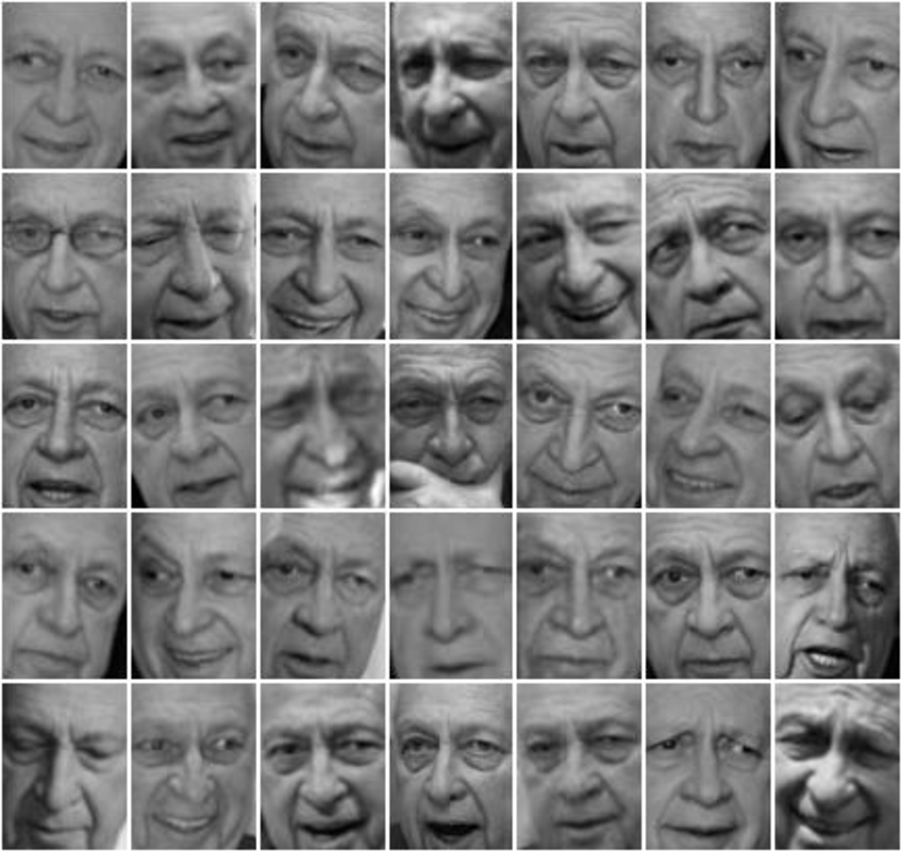
\includegraphics[width=0.5\textwidth]{../figures/rasl_original.pdf}}
  ~
  \subfloat[Aligned images $M\circ\tau$]{\label{fig:rasl:aligned}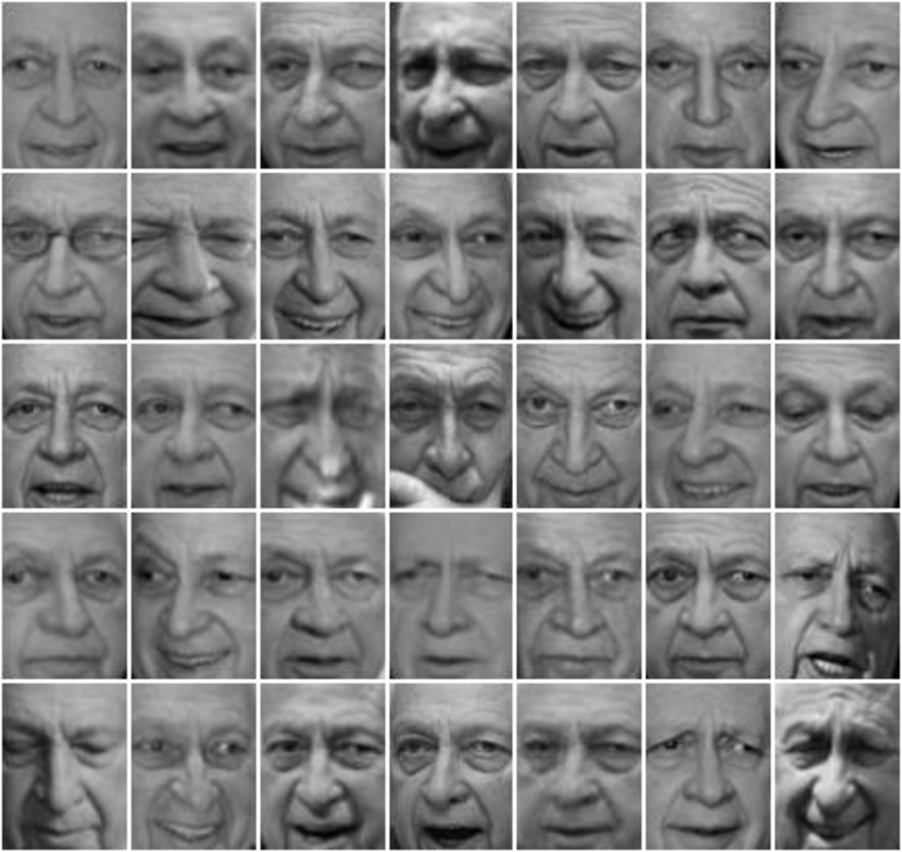
\includegraphics[width=0.5\textwidth]{../figures/rasl_aligned.pdf}}
  ~
  \\ \subfloat[Low-rank component $L$]{\label{fig:rasl:lowrank}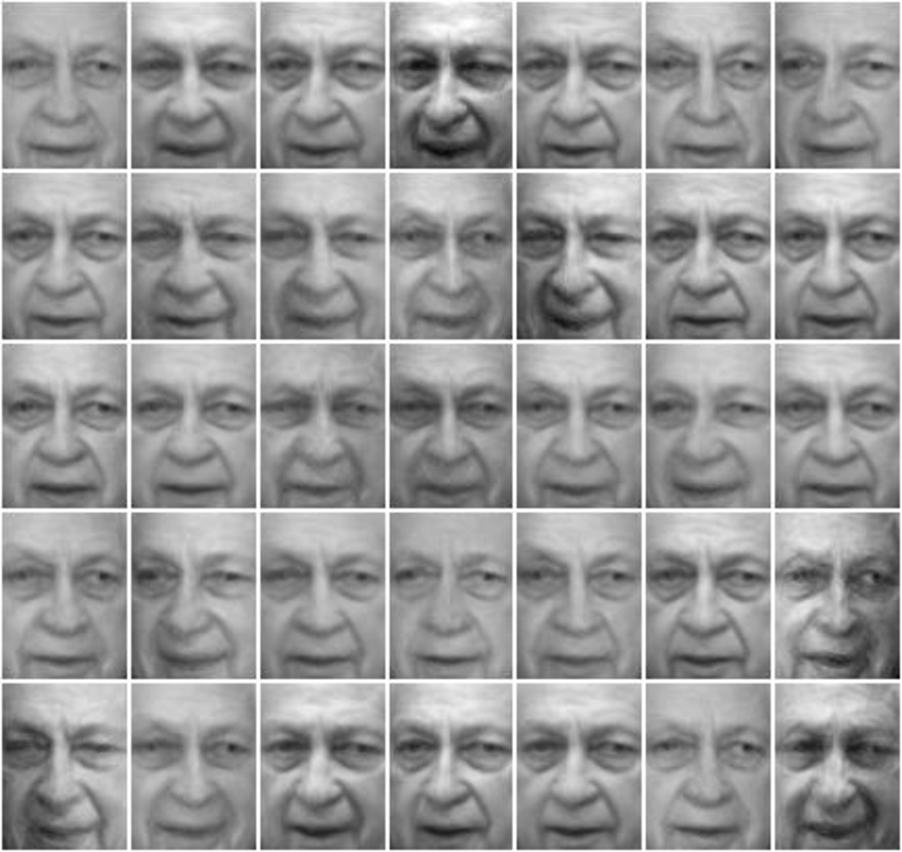
\includegraphics[width=0.5\textwidth]{../figures/rasl_low_rank.pdf}}
  ~
  \subfloat[Sparse component $S$]{\label{fig:rasl:sparse}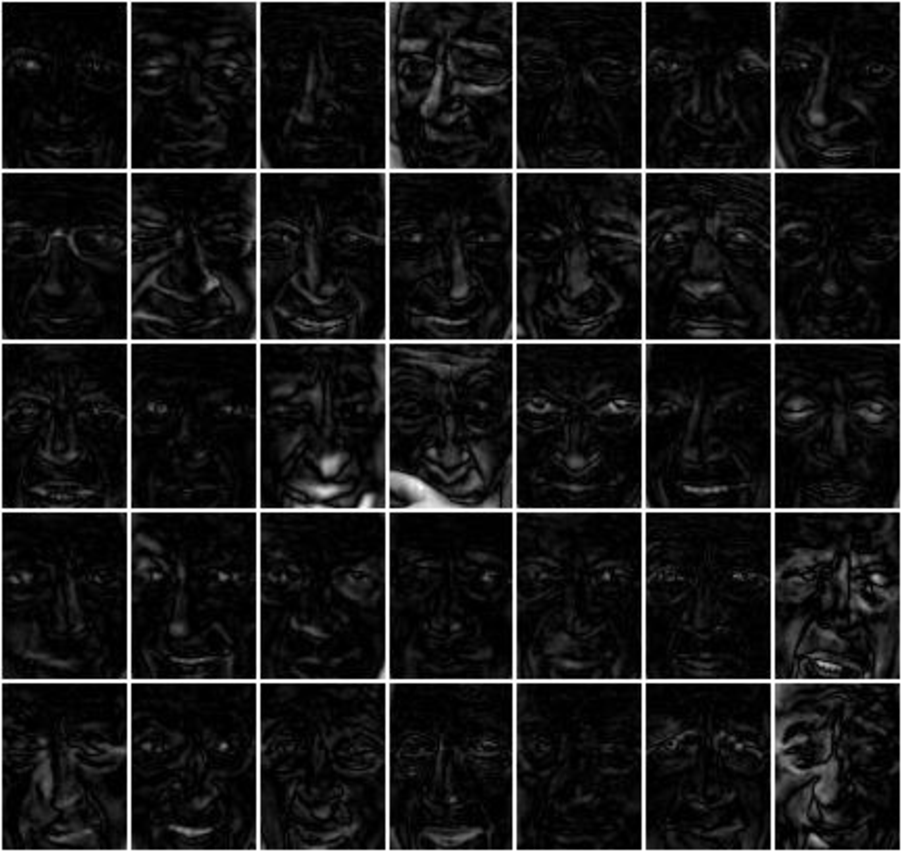
\includegraphics[width=0.5\textwidth]{../figures/rasl_sparse.pdf}}

  \caption{Aligning face images.}
  \label{fig:rasl:example}
\end{figure}



%-----------------------------------------------------------------------------------------------------------------------------------------------------------------
\subsection{Robust Matrix Decomposition With Sparse Corruptions}
\subsubsection{Introduction}

In the problem of solving Robust PCA, exact recovery via convex optimization of the $\ell_{1}$ and nuclear norm heuristic is possible with high probability if the sparse noise is evenly spread out. However, in some applications, the sparse noise may not be evenly spread out and we are satisfied as long as the recovered matrix is sufficiently close with the original matrix. Therefore, the authors~\cite{Hsu:2011ys} analyze the Robust PCA problem in a deterministic setting without assuming a particular sparsity pattern of the noise. They give sufficient conditions on the level of sparsity that is required for a tolerable recovery of the sparse and low-rank pairs.


\subsubsection{Main ideas and contributions}
%
Similar to the prior study of Robust PCA, the authors of~\cite{Hsu:2011ys} study a minimization
of a weighted combination of $\ell_{1}$ and nuclear norm . However, they also introduce some tolerance on the perturbation in the constraints. In particular, given the observed matrix~$M$ (a perturbed observation of the original $(L_{0},S_{0})$ pairs), they analyze the following two optimization problems: % With arguments as $(L,S)$,
%
\begin{eqnarray}
\min_{(L,S)} & \|L\|_{*}+\lambda\|S\|_{1}\nonumber \\
s.t. & \|L+S-M\|_{1}\le\epsilon_{1}\\
 & \|L+S-M\|_{*}\le\epsilon_{*}\nonumber
\end{eqnarray}
%
and the regularized version
\begin{eqnarray}
\min_{(L,S)} & \|L\|_{*}+\lambda\|S\|_{1}+\frac{1}{2\mu}\|L+S-M\|_{F}
\end{eqnarray}


The authors provide sufficient conditions on the pair $(L_{0},S_{0})$ that allow accurate recovery in the sense that $\|L_{0}-\hat{L}\|_{\infty},\|S_{0}-\hat{S}\|_{\infty}$ is small. Moreover, they show that if the observed matrix~$M$ is perturbed from $L_{0}+S_{0}$ by a small amount (i.e. $\epsilon$), the optimizer $(\hat{L},\hat{S})$ will still be $\epsilon$-close to the original $(L_{0},S_{0})$ pair. As in Robust PCA, the key ideas of the analysis of the performance guarantee is based on the properties of the constructed dual certificate.

\subsubsection{Discussion and applications}
The work~\cite{Hsu:2011ys} parallels the work of~\cite{Candes:2011fk} but gives a weaker guarantee in a deterministic setting. %Although not pointed out by the authors, 
We believe that the performance guarantee in this~\cite{Hsu:2011ys} and related work is also useful in many applications. For example, in computer vision, the noise  is normally clustered at some portion of the image and it is not natural to assume the noise to be uniformly distributed. Moreover, in many real world applications, we are often satisfied with approximate recovery. %instead of exact recovery, so the study of perturbed version is needed. 
For example, in many analyses of large data sets (say for example consumer ranking in Netflix), we are interested in the general idea of the pattern but not necessarily the fine details. At this point it is still unclear whether the sufficient conditions provided for the perturbed problem are also necessary. %It would be nice if there is any progress towards this end. 




%-----------------------------------------------------------------------------------------------------------------------------------------------------------------
%-----------------------------------------------------------------------------------------------------------------------------------------------------------------
\subsection{Structured Sparsity}
In~\cite{Bach:2011kx}, the authors present an overview of techniques that extend the idea of $\ell_1$ regularization, to induce structured sparsity. The idea is to use structured-sparsity-inducing norms to encourage some sparsity patterns over others, given some a priori information on the expected or desired sparsity pattern of the solution. For instance, in feature selection problems, one may have groups of features that are highly correlated, and would like features that belong to the same group to be either all in the support, or all outside of the support. Another example is shadow elimination from images, where one expects shadows to be connected and to have spacial structure.


\subsubsection{Structured-sparsity-inducing norms}
Consider in particular the regularized learning problem
\begin{equation}
\label{eq:struct_spars}
\min_{w \in \Rbb^p} f(w) = \min_{w \in \Rbb^p} \frac{1}{n} \sum_{i = 1}^n L(y^{(i)} + w^Tx^{(i)}) + \lambda \Omega(w)
\end{equation}
where $\ell$ is a differentiable loss function, $(x^{(i)}, y^{(i)})$ is the training data, $w$ is the regression vector, and $\Omega$ is a norm. We are interested in norms that not only induce sparsity, but also have a structure in their support, for example by having groups of variables that are selected or ignored simultaneously. A natural idea is to partition the variables into such groups, which leads to sparsity with disjoint groups of variables

\paragraph{Disjoint groups of variables an group Lasso}
Assume the feature set is partitioned into a collection $\mathcal{G}$. Then the structure sparsity norm $\Omega$ is defined as
\[
\Omega(w)  = \sum_{g \in \mathcal{G}} \|w_g\|_q
\]

where $q \in (1, \infty]$, i.e. $\|.\|_q$ is any norm (usually $\|.\|_2$ or $\|.\|_\infty$). In the context of least square regression, this regularization is known as the group Lasso. As expected, experimental results reported in~\cite{Bach:2011kx} show that variables in the same group are either all set to zero (all outside the support), or all selected (all in the support).

\paragraph{Overlapping groups of variables}
Using overlapping groups (when elements of $\mathcal{G}$ are not necessarily disjoint) allows for more flexibility and more complex structures. For example, in image processing (shadow removal, background extraction) where pixels are arranged on a grid, using groups formed by one pixel and his neighbors yields good results in background extraction~\cite{Cevher_sparsesignal}.


\paragraph{Proximal method}
Proximal methods take advantage of the form~\ref{eq:struct_spars} as a sum of two convex terms, a smooth term and a term for which computing the proximal gradient is cheap. Proximal methods are iterative procedure, where at each iteration, the function $f$ is linearized around the current estimate $w$, and update the estimate by the unique solution of the optimization problem
\[
w_+ = \arg \min_{w \in \Rbb^p} f(\hat{w}) + (w - \hat{w})^T\nabla f(\hat{w}) + \lambda \Omega(w) + \frac{L}{2}\|w - \hat{w}\|_2^2
\]

where the parameter $L$ is an upper bound on the Lipschitz constant of $\nabla f$. This can be rewritten as
\[
w_+ = \arg \min_{w \in \Rbb^p} \frac{1}{2} \left\|w - \left( \hat{w} - \frac{1}{L} \nabla f(\hat{w}) \right) \right\|_2^2 + \frac{\lambda}{L} \Omega(w)
\]
which is an instance of the proximal operator
\[
\text{Prox}_{\lambda \Omega} : u \mapsto \underset{v \in \Rbb^p }{\arg \min} \frac{1}{2}\|u - v\|_2^2 + \lambda \Omega(v)
\]
and it turns out that the proximal operator can be computed exactly for many structured-sparsity-inducing norms. Note in particular that when $\Omega$ is the $\ell_1$ norm, the proximal operator is the soft thresholding operator.

